\graphicspath{{img/results}{img/results/out}}

\chapter{Results}
\label{ch:results}
This chapter will present the results of the smarticle experiments in the TASEP. We will start by setting a baseline with the classical TASEP and analyze how different speed distributions affect this purely stochastic system. Next, we will compare the results with a simple hard-coded policy, before moving on to the smarticle training. We will analyze the results of the smarticle training for different reward structures and compare them to the baseline. 

\section{Setting a Baseline: Classical TASEP}
\label{sec:baseline}
This section will use the classical 2D (T)ASEP as introduced in section \ref{sec:2d-tasep}. We will make it totally asymmetric in the horizontal direction (the \textit{forward} direction) by setting the probability $p$ to jump forward to $1/2$ and the probability $q$ to jump backward to $0$. The vertical direction (the \textit{up/down} direction) will be symmetric with probabilities $a=b=1/4$. The system has periodic boundary conditions in both directions. We will analyze a $128 \times 32$ system and a narrower $128 \times 6$ system. Both systems will be initialized with a checkerboard pattern of particles and holes, yielding a density of $\rho = 1/2$. This density will be chosen for most experiments, as it is dense enough for the different policies and speed distributions to have a significant effect on the system, but not so dense that the system is always jammed. Speeds will be drawn from a truncated normal distribution with mean $0.5$ and different standard deviations $\sigma$. The distribution is truncated at $0$ and $1$, so that speeds are always in that range. Two example speed distributions are shown in figure \ref{fig:speed_dists}. 
\begin{figure}
    \centering
    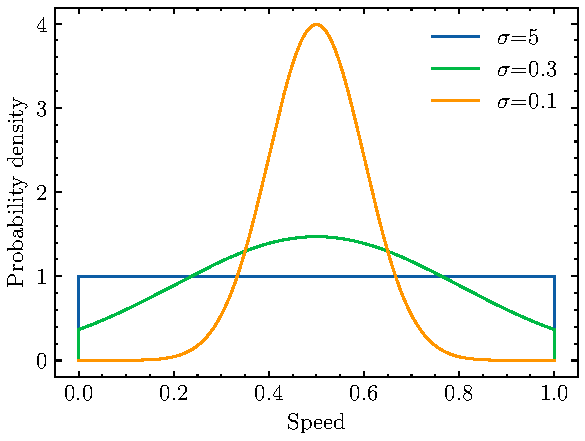
\includegraphics{truncated_normal.pdf}
    \caption{Normalized truncated normal distributions with mean $0.5$ different standard deviations $\sigma$. For $\sigma = 5$, the distribution is almost uniform.}
    \label{fig:speed_dists}
\end{figure}

\begin{figure}
    \centering
    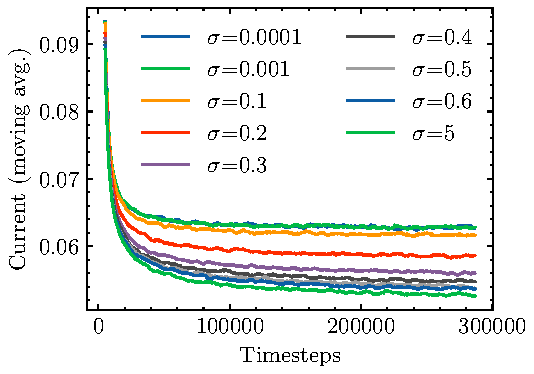
\includegraphics{currents_fixed_sigma.pdf}
    \caption{Current as a function of time steps since initialization of the system to the checkerboard pattern for different speed distribution standard deviations $\sigma$. The data is averaged over 800 independent runs and plotted with a moving average over 5000 time steps.}
    \label{fig:currents_fixed_sigma_128x32}
\end{figure}

\begin{figure}
    \centering
    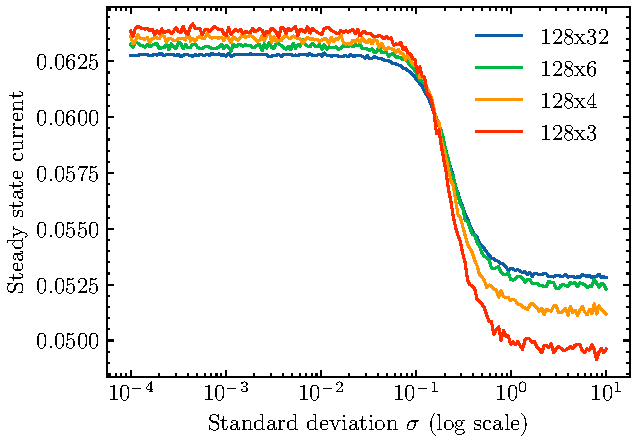
\includegraphics{steady_state_current_sizes_log.pdf}
    \caption{Steady state current as a function of the speed distribution standard deviation $\sigma$ for different system sizes. Steady state current is calculated as the average current over all remaining time steps after the steady state has been reached (the current has stopped dropping). The data is averaged over 800 independent runs.}
    \label{fig:steady_state_current_sizes_log}
\end{figure}

\begin{figure}
    \centering
    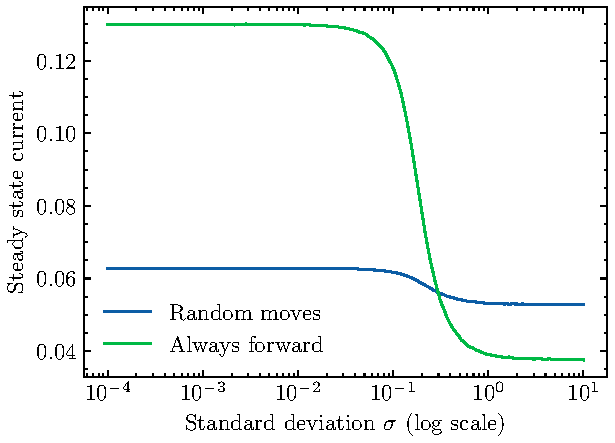
\includegraphics{steady_state_current_both_log.pdf}
    \caption{}
    \label{fig:steady_state_current_always_forward}
\end{figure}
